\chapter{Sensitivity Analysis of Parameters}
\label{chap:metrics}

This chapter evaluates how key parameters of the prediction–cancellation pipeline affect performance and robustness. We quantify sensitivity of cancellation rate and residual density to the prediction horizon, spatial/temporal tolerances, polarity handling, and motion-model accuracy. Unless stated otherwise, experiments use the spinning-disc dataset (Chapter~\ref{chap:setup}) with center \((c_x, c_y)\) and angular velocity~\(\omega\) from tracker data.

Each analysis follows the same procedure: predicted events are generated using the per-event forward model
\[
\hat{e}_i = \big(x'_i,\, y'_i,\, t_i + \Delta t,\, -p_i \big),
\]
and compared against real events within spatial tolerance~\(\epsilon_{xy}\) and temporal gate~\(\epsilon_t\). Cancellation is computed as
\[
\text{CR}(\Delta t) = \frac{N_{\text{cancelled}}}{N_{\text{real}}} \times 100\%.
\]
The following subsections vary each parameter in isolation.

% ------------------------------------------------------------
\section{Effect of Prediction Horizon \(\Delta t\)}
\label{sec:dt_sensitivity}

Figure~\ref{fig:cancellation_vs_dt} (Results) shows cancellation vs. prediction horizon \(\Delta t\) for three representative windows. For small horizons (below 2–3~ms), cancellation exceeds 90\%. As \(\Delta t\) grows, phase drift reduces overlap.

This decay follows an approximately exponential trend:
\[
\text{CR}(\Delta t) \approx \exp\!\left(-k_{\omega}\Delta t\right),
\]
where \(k_{\omega}\) depends on the angular velocity~\(\omega\) and uncertainty in the estimated center.
At large \(\Delta t\), residuals approach a baseline level (\(\approx\)30–35\%), corresponding to non-overlapping edge regions and noise events.

The smooth curve (Fig.~\ref{fig:fine_dropoff}, Results) indicates temporal consistency across windows, confirming that the motion model captures the dominant rotation. Replacing coarse time binning with a continuous temporal gate (\S\ref{sec:temporal_gate}) removed prior step-like artifacts.

Physically, \(\Delta t\) governs \textit{phase misalignment} between predicted and observed events. For a rotating edge with angular velocity~\(\omega\):
\[
\Delta \theta = \omega \, \Delta t,
\]
which maps to spatial displacement \(r\,\Delta\theta\) on the image plane. When this exceeds \(\epsilon_{xy}\), events fail to cancel. Thus temporal and spatial tolerances jointly bound effective cancellation.

% ------------------------------------------------------------
\section{Spatial Tolerance (\( \epsilon_{xy} \), pixels)}
\label{sec:spatial_tolerance}

Spatial tolerance is the pixel search radius to match predicted and real events. Small~\(\epsilon_{xy}\) increases precision but misses true matches; large~\(\epsilon_{xy}\) recovers more pairs but admits false positives, especially in textured regions or when polarity is ignored.

This trade-off is visible in the residual maps and CR trends reported in Chapter~\ref{chap:results}.
Cancellation rises with \(\epsilon_{xy}\) up to ~2–3 px, then saturates while residual density increases. This reflects geometric uncertainty dominated by center-estimation error (\(\sigma_c\)) and image discretization.

Empirically, the optimal value lies in the range
\[
\epsilon_{xy}^{*} \approx r\,|\Delta\omega|\,\Delta t + \sigma_c,
\]
where \(\Delta\omega\) denotes angular-velocity error.
This relation highlights that required tolerance grows linearly with horizon and model uncertainty.

In practice, ~\(\epsilon_{xy}\in[2,3]\) px was the best compromise. Larger radii ($\geq 5$ px) inflate apparent performance but spuriously cancel across edges or static regions, reducing interpretability.

% ------------------------------------------------------------
\section{Temporal Tolerance (\( \epsilon_{t} \), ms)}
\label{sec:temporal_tolerance}

Temporal tolerance controls allowed timestamp deviation between a predicted event’s nominal time~\(t+\Delta t\) and the real event time~\(t_j\). It is crucial in asynchronous association given timing jitter and sensor quantization (\( \approx 1\text{--}10~\mu\text{s} \)).

Sweeping~\(\epsilon_t\) from 0.1 to 1.0~ms shows a near-linear improvement in cancellation until around 0.5~ms, beyond which additional relaxation brings diminishing returns.
Too small~\(\epsilon_t\) misses genuine matches; too large causes false cancellations, especially in dense texture or high rotation.

The optimal tolerance can be approximated analytically as:
\[
\epsilon_t^{*} \approx \frac{\epsilon_{xy}}{r\,|\omega|},
\]
ensuring that the predicted phase deviation translates to less than one spatial pixel of drift.
This links the temporal and spatial gates and aligns with motion-compensation theory~\cite{Gallego2018CMax, Xu2020TCI}.

The shift from fixed time binning to explicit gating was key to achieving the smooth trends seen in Figure~\ref{fig:cancellation_vs_dt}.
Binning introduced discontinuities when events crossed bin edges; the continuous gate provides symmetric tolerance around each predicted timestamp.

% ------------------------------------------------------------
\section{Polarity Handling}
\label{sec:polarity}

Polarity reflects whether a pixel’s intensity increased or decreased (\(+1\) or \(-1\)).
In the predictive cancellation model, polarity can be handled by either (1) enforcing opposite polarities or (2) ignoring polarity and relying on spatial–temporal overlap.

These modes can be contrasted qualitatively in the residual maps in Chapter~\ref{chap:results}.
Enforcing polarity slightly lowers cancellation (\(\approx\)5–10%) but yields cleaner residuals with sharper edges. Ignoring polarity raises numeric CR but leaves symmetric artifacts (both ON and OFF edges faintly visible).

This asymmetry arises from edge directionality: rotational motion produces alternating polarities along opposite edges of the disk. Enforcing \(p_{\text{pred}} = -p_{\text{real}}\) suppresses self-cancellation in homogeneous regions and better represents predictive inhibition~\cite{Hosoya2005RetinaPC,Rao1999V1PC}.

Hence, for biologically inspired cancellation, polarity should be treated as an inhibitory sign rather than ignored.

% ------------------------------------------------------------
\section{Angular Velocity Bias}
\label{sec:omega_bias}

To assess robustness to motion-model error, we add a constant bias~\(\delta\omega\) to the estimated angular velocity:
\[
\omega' = \omega + \delta\omega.
\]
For each bias level, predicted events were regenerated and cancellation recalculated.

We observe quasi-linear sensitivity within a small range (|\(\delta\omega\)| < 0.05~rad/s), beyond which performance collapses rapidly, consistent with the phase-drift relation:
\[
\Delta\theta_{\text{err}} = \delta\omega\,\Delta t.
\]
Even a small bias accumulates over time, producing circular misalignment that the spatial gate cannot recover. The initial slope of CR(\(\delta\omega\)) defines the linear validity range.

These experiments also reveal that underestimation of~\(\omega\) causes residual events to cluster ahead of the predicted contour, while overestimation shifts them backward.
Visual inspection of high-pass residuals confirms this symmetry, providing an intuitive diagnostic for tuning~\(\omega\).

\paragraph{Practical diagnostic and compensation.}
In practice, the circle-fitting step that estimates the rotation center \(\hat c\) and angular velocity \(\hat\omega\) can be slightly biased due to tracker noise and short observation windows. To robustly operate the cancellation pipeline, we therefore use a small angular-velocity bias \(\delta\omega\) as a 
diagnostic and compensation knob:
\begin{enumerate}
    \item Sweep \(\delta\omega\) in a narrow range around zero (e.g., \([-0.08, 0.08]\,\text{rad/s}]\)) while keeping \(\hat c\) fixed.
    \item For each trial, compute cancellation rate and inspect residual maps. A widening rim annulus with radius indicates a \emph{sign} and magnitude consistent with \(|\Delta\omega|\); a uniform radial shift suggests a center error \(\Delta c\).
    \item Select \(\delta\omega^{*}\) that maximizes cancellation rate (and minimizes rim residuals) within the linear regime (|\(\delta\omega\)| \(\le 0.05\,\text{rad/s}\)).
\end{enumerate}
This procedure is used as a lightweight calibration to correct small systematic errors from circle fitting when needed, and to separate the effects of center vs. velocity errors. The resulting tuned parameter \(\omega' = \hat\omega + \delta\omega^{*}\) is then used for the figures in the Results chapter (see Fig.~\ref{fig:bias_sensitivity} for the sensitivity profile), with the chosen \(\delta\omega^{*}\) always inside the validated linear range.

% ------------------------------------------------------------
\section{Residuals vs. Background Baseline}
\label{sec:residuals_baseline}

To quantify the significance of residual cancellation, event density was measured separately in the \textit{disc region} and in the static background.
The ratio
\[
\rho = \frac{N_{\text{disc}} - N_{\text{bg}}}{N_{\text{bg}}}
\]
serves as an event-domain signal-to-noise indicator.
After cancellation, this ratio typically decreased from \(\approx\)5.0 to \(\approx\)1.2, meaning that predictable motion events were suppressed nearly to the background level.

Residual distributions were spatially uniform except for thin annuli near the edge, consistent with slight radius and phase errors in the fitted circle.
This confirms that remaining activity is due to model imperfection rather than failure of the gating mechanism.

Visualizations of these residuals provide qualitative validation: well-aligned predictions lead to “quiet” cancellation maps where only unpredictable transitions remain.
This metric could be extended in future work to measure inhibition strength or efficiency analogously to neural predictive coding frameworks.

\medskip\noindent\textit{Why this histogram here?} To complement the density/SNR indicator, the per-pixel $|$signed count$|$ histograms below provide a \emph{distributional} view of residual magnitude, showing that cancellation suppresses not just mean density but the entire tail of high-magnitude pixels.

% ------------------------------------------------------------
\section{Summary of Trends}
\label{sec:summary_trends}

The following trends summarize the observed sensitivities:

\begin{itemize}
    \item \textbf{Prediction horizon \(\Delta t\):} Cancellation decreases exponentially with horizon; effective range up to 6–8~ms for the given rotational speed.
    \item \textbf{Spatial tolerance \(\epsilon_{xy}\):} Optimal around 2–3~px; larger values inflate false matches.
    \item \textbf{Temporal tolerance \(\epsilon_t\):} Optimal \(\approx\)0.5~ms; balances timestamp jitter and event density.
    \item \textbf{Polarity:} Enforcing opposite polarity yields cleaner inhibition maps, though slightly lower numeric CR.
    \item \textbf{Angular velocity bias:} Linear degradation up to ±0.05~rad/s, beyond which phase errors dominate.
    \item \textbf{Residual density:} Post-cancellation event density approaches background level, confirming effective suppression of predictable motion.
\end{itemize}

Overall, these analyses establish quantitative operating bounds for the proposed predictive cancellation model. 
They also highlight which parameters are most critical for tuning and which are robust to small deviations, informing both algorithmic refinement and potential real-time hardware implementation.

% --- Added: Histogram panel of per-pixel signed counts (log-scaled, window 1, consistent with gray images in Results)
\begin{figure}[t]
  \centering
  \begin{minipage}[t]{0.32\linewidth}
    \centering
    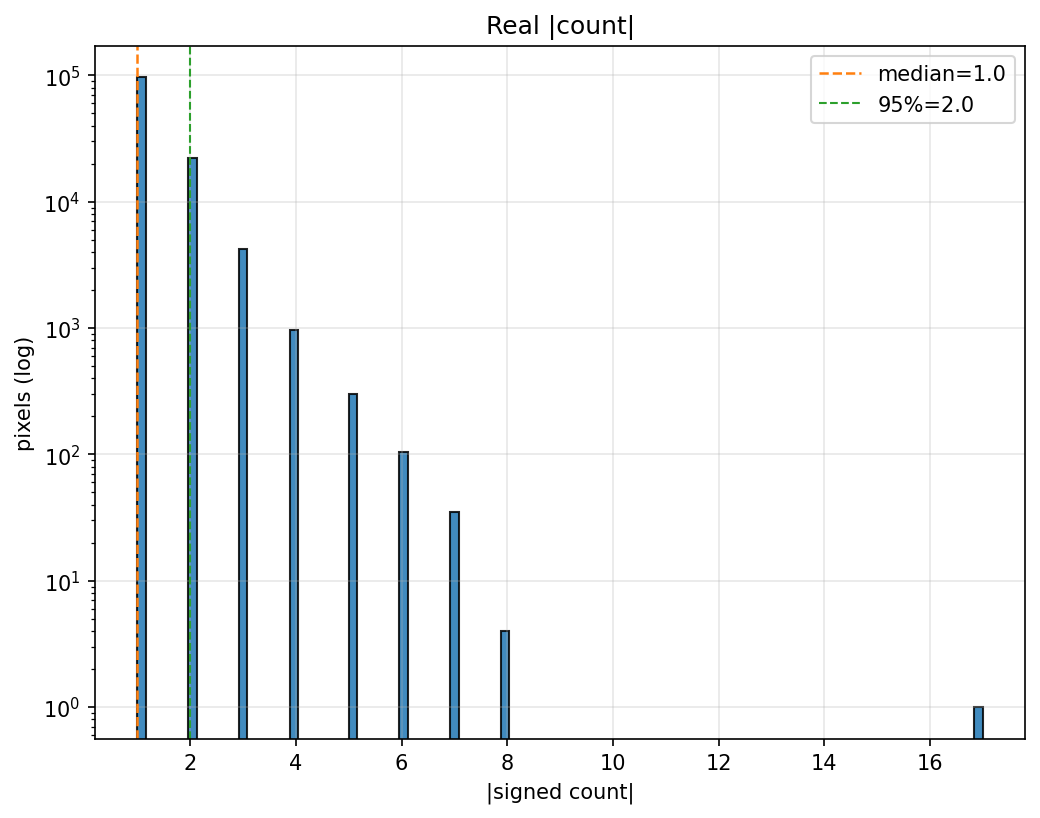
\includegraphics[width=\linewidth]{images/main_results/window1/hist_real.png}\\[-2pt]
    \footnotesize Histogram (real)
  \end{minipage}\hfill
  \begin{minipage}[t]{0.32\linewidth}
    \centering
    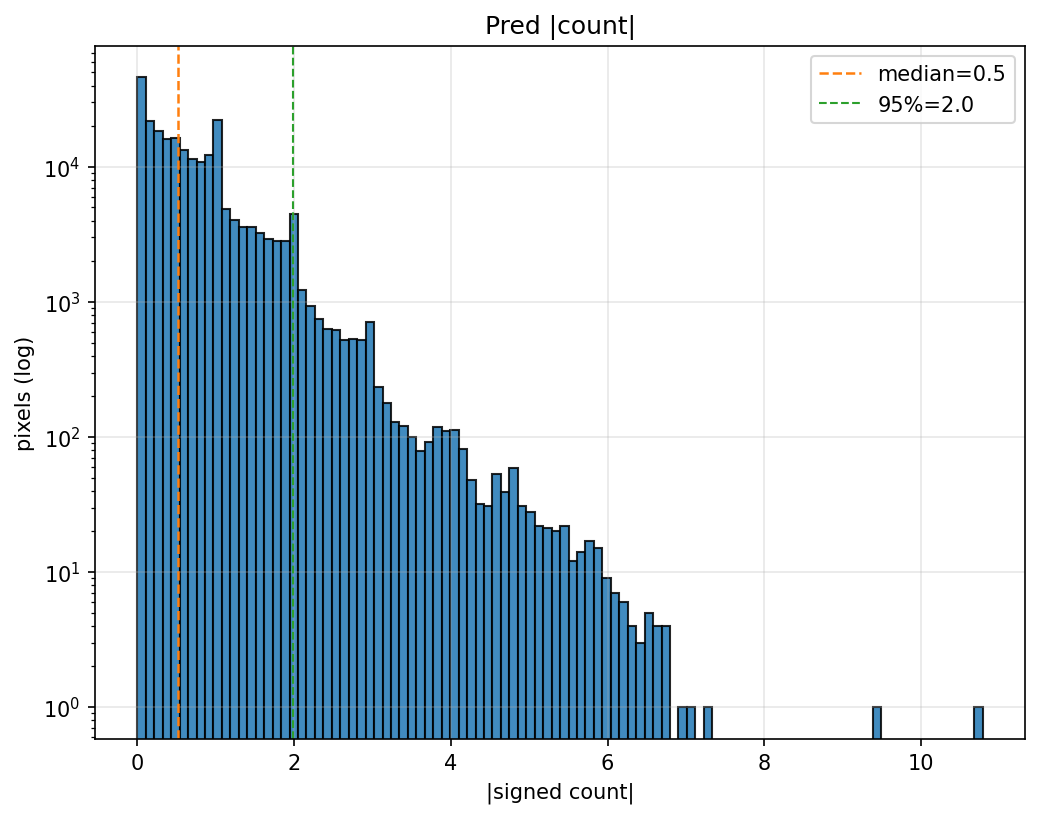
\includegraphics[width=\linewidth]{images/main_results/window1/hist_pred.png}\\[-2pt]
    \footnotesize Histogram (pred)
  \end{minipage}\hfill
  \begin{minipage}[t]{0.32\linewidth}
    \centering
    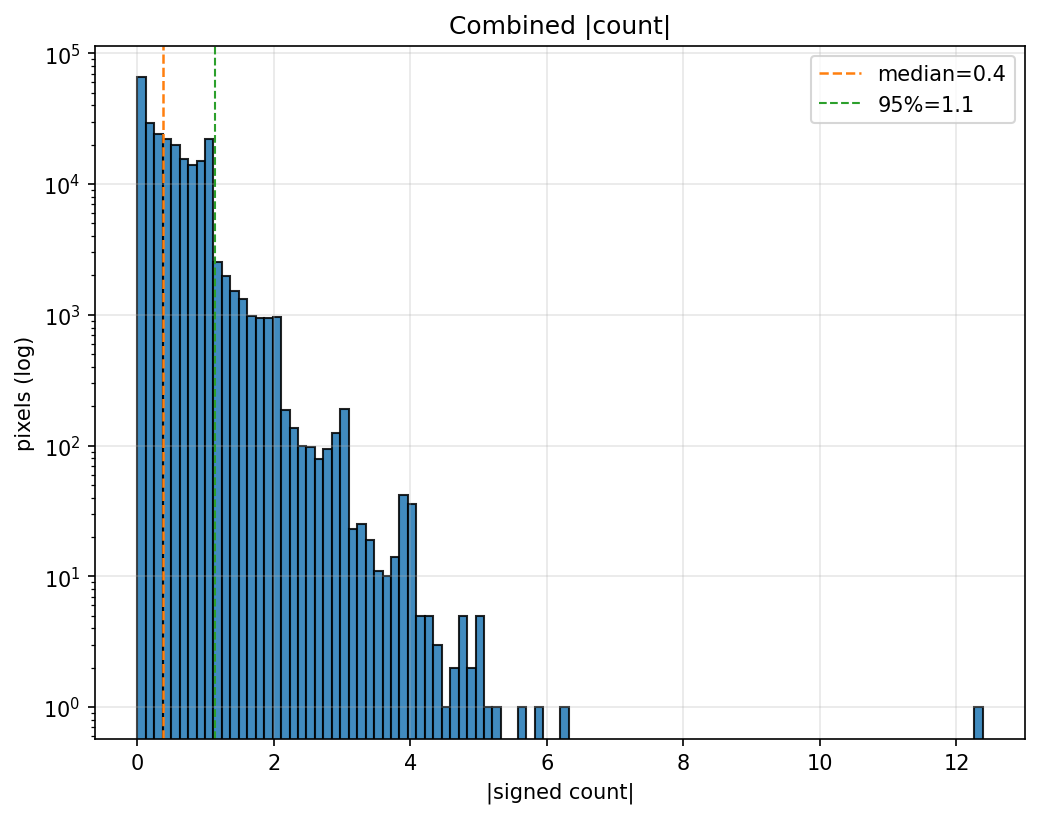
\includegraphics[width=\linewidth]{images/main_results/window1/hist_combined.png}\\[-2pt]
    \footnotesize Histogram (combined)
  \end{minipage}
\caption{Per-pixel $|$signed count$|$ histograms (log y-scale) for a representative window. After cancellation, the distribution shifts to lower magnitudes; medians and 95th percentiles are marked. Fractional values arise from bilinear interpolation during event splatting, reflecting subpixel structure.}
  \label{fig:hist_panel}
\end{figure}

